%%%%%%%%%%%%%%%%%%%%%%%%%%%%%%%%%%%%%%%%%
% Quality Report Format from
% Derived from The Legrand Orange Book LaTeX Template (Overleaf)
%%%%%%%%%%%%%%%%%%%%%%%%%%%%%%%%%%%%%%%%%



% When you first open the template, compile it from the command line with the 
% commands below to make sure your LaTeX distribution is configured correctly:
% Re-run to get TOC
% 1) pdflatex main
% 2) makeindex main.idx -s StyleInd.ist
% 3) biber main
% 4) pdflatex main x 2

%%%%%%%%%%%%%%%%%%%%%%%%%%%%%%%%
%GRAPHICS
%%%%%%%%%%%%%%%%%%%%%%%%%%%%%%%%%
% graphics for cover photo and chapter photos must be .jpeg



%----------------------------------------------------------------------------------------
%	PACKAGES AND OTHER DOCUMENT CONFIGURATIONS
%----------------------------------------------------------------------------------------

\documentclass[11pt,fleqn]{book} % Default font size and left-justified equations

\usepackage[top=3cm,bottom=3cm,left=3.2cm,right=3.2cm,headsep=10pt,letterpaper]{geometry} % Page margins
\usepackage{lipsum}
\usepackage{xcolor} % Required for specifying colors by name
\definecolor{ocre}{RGB}{51,102,0} 
\definecolor{lightgray}{RGB}{229,229,229}
\usepackage{csquotes}


% Font Settings
\usepackage{avant} % Use the Avantgarde font for headings
%\usepackage{times} % Use the Times font for headings
\usepackage{mathptmx} % Use the Adobe Times Roman as the default text font together with math symbols from the Sym­bol, Chancery and Com­puter Modern fonts

\usepackage{microtype} % Slightly tweak font spacing for aesthetics
\usepackage[utf8]{inputenc} % Required for including letters with accents
\usepackage[T1]{fontenc} % Use 8-bit encoding that has 256 glyphs


% MATHS PACKAGE
\usepackage{amsmath}
\usepackage{calc}

% GRAPHICS
\usepackage{tikz}
\usetikzlibrary{matrix}
\newcommand*{\horzbar}{\rule[0.05ex]{2.5ex}{0.5pt}}


% VERBATIM PACKAGE
\usepackage{verbatim}



% BIBLIOGRAPHY
\usepackage[american]{babel} 
\usepackage[style=apa,
            sorting=nyt,
            sortcites=true,
            autopunct=true,
            hyperref=true,
            maxcitenames=2,
            mincitenames=1,
            maxbibnames=10,
            backref=true,
            doi=false,
            url=false,
            backend=biber]{biblatex}
\addbibresource{/home/bruce/Desktop/BibLatex/My_Library_20170125.bib} % BibTeX bibliography file
%\defbibheading{bibempty}{}
\DeclareLanguageMapping{american}{american-apa}    % avoid yearmonthday problems


% INDEX
\usepackage{imakeidx}
\makeindex



%----------------------------------------------------------------------------------------
%	VARIOUS REQUIRED PACKAGES
%----------------------------------------------------------------------------------------

\usepackage{titlesec} % Allows customization of titles

\usepackage{graphicx} % Required for including pictures
\graphicspath{{Pictures/}} % Specifies the directory where pictures are stored

\usepackage{lipsum} % Inserts dummy text

\usepackage{tikz} % Required for drawing custom shapes

\usepackage[english]{babel} % English language/hyphenation

\usepackage{enumitem} % Customize lists
\setlist{nolistsep} % Reduce spacing between bullet points and numbered lists

\usepackage{booktabs} % Required for nicer horizontal rules in tables

\usepackage{eso-pic} % Required for specifying an image background in the title page

%----------------------------------------------------------------------------------------
%	MAIN TABLE OF CONTENTS
%----------------------------------------------------------------------------------------

\usepackage{titletoc} % Required for manipulating the table of contents

\contentsmargin{0cm} % Removes the default margin
% Chapter text styling
\titlecontents{chapter}[1.25cm] % Indentation
{\addvspace{15pt}\large\sffamily\bfseries} % Spacing and font options for chapters
{\color{ocre!60}\contentslabel[\Large\thecontentslabel]{1.25cm}\color{ocre}} % Chapter number
{}  
{\color{ocre!60}\normalsize\sffamily\bfseries\;\titlerule*[.5pc]{.}\;\thecontentspage} % Page number
% Section text styling
\titlecontents{section}[1.25cm] % Indentation
{\addvspace{5pt}\sffamily\bfseries} % Spacing and font options for sections
{\contentslabel[\thecontentslabel]{1.25cm}} % Section number
{}
{\sffamily\hfill\color{black}\thecontentspage} % Page number
[]
% Subsection text styling
\titlecontents{subsection}[1.25cm] % Indentation
{\addvspace{1pt}\sffamily\small} % Spacing and font options for subsections
{\contentslabel[\thecontentslabel]{1.25cm}} % Subsection number
{}
{\sffamily\;\titlerule*[.5pc]{.}\;\thecontentspage} % Page number
[] 

%----------------------------------------------------------------------------------------
%	MINI TABLE OF CONTENTS IN CHAPTER HEADS
%----------------------------------------------------------------------------------------

% Section text styling
\titlecontents{lsection}[0em] % Indendating
{\footnotesize\sffamily} % Font settings
{}
{}
{}

% Subsection text styling
\titlecontents{lsubsection}[.5em] % Indentation
{\normalfont\footnotesize\sffamily} % Font settings
{}
{}
{}
 
%----------------------------------------------------------------------------------------
%	PAGE HEADERS
%----------------------------------------------------------------------------------------

\usepackage{fancyhdr} % Required for header and footer configuration

\pagestyle{fancy}
\renewcommand{\chaptermark}[1]{\markboth{\sffamily\normalsize\bfseries\chaptername\ \thechapter.\ #1}{}} % Chapter text font settings
\renewcommand{\sectionmark}[1]{\markright{\sffamily\normalsize\thesection\hspace{5pt}#1}{}} % Section text font settings
\fancyhf{} \fancyhead[LE,RO]{\sffamily\normalsize\thepage} % Font setting for the page number in the header
\fancyhead[LO]{\rightmark} % Print the nearest section name on the left side of odd pages
\fancyhead[RE]{\leftmark} % Print the current chapter name on the right side of even pages
\renewcommand{\headrulewidth}{0.5pt} % Width of the rule under the header
\addtolength{\headheight}{2.5pt} % Increase the spacing around the header slightly
\renewcommand{\footrulewidth}{0pt} % Removes the rule in the footer
\fancypagestyle{plain}{\fancyhead{}\renewcommand{\headrulewidth}{0pt}} % Style for when a plain pagestyle is specified

% Removes the header from odd empty pages at the end of chapters
\makeatletter
\renewcommand{\cleardoublepage}{
\clearpage\ifodd\c@page\else
\hbox{}
\vspace*{\fill}
\thispagestyle{empty}
\newpage
\fi}

%----------------------------------------------------------------------------------------
%	THEOREM STYLES
%----------------------------------------------------------------------------------------

\usepackage{amsmath,amsfonts,amssymb,amsthm} % For math equations, theorems, symbols, etc

\newcommand{\intoo}[2]{\mathopen{]}#1\,;#2\mathclose{[}}
\newcommand{\ud}{\mathop{\mathrm{{}d}}\mathopen{}}
\newcommand{\intff}[2]{\mathopen{[}#1\,;#2\mathclose{]}}
\newtheorem{notation}{Notation}[chapter]

%%%%%%%%%%%%%%%%%%%%%%%%%%%%%%%%%%%%%%%%%%%%%%%%%%%%%%%%%%%%%%%%%%%%%%%%%%%
%%%%%%%%%%%%%%%%%%%% dedicated to boxed/framed environements %%%%%%%%%%%%%%
%%%%%%%%%%%%%%%%%%%%%%%%%%%%%%%%%%%%%%%%%%%%%%%%%%%%%%%%%%%%%%%%%%%%%%%%%%%
\newtheoremstyle{ocrenumbox}% % Theorem style name
{0pt}% Space above
{0pt}% Space below
{\normalfont}% % Body font
{}% Indent amount
{\small\bf\sffamily\color{ocre}}% % Theorem head font
{\;}% Punctuation after theorem head
{0.25em}% Space after theorem head
{\small\sffamily\color{ocre}\thmname{#1}\nobreakspace\thmnumber{\@ifnotempty{#1}{}\@upn{#2}}% Theorem text (e.g. Theorem 2.1)
\thmnote{\nobreakspace\the\thm@notefont\sffamily\bfseries\color{black}---\nobreakspace#3.}} % Optional theorem note
\renewcommand{\qedsymbol}{$\blacksquare$}% Optional qed square

\newtheoremstyle{blacknumex}% Theorem style name
{5pt}% Space above
{5pt}% Space below
{\normalfont}% Body font
{} % Indent amount
{\small\bf\sffamily}% Theorem head font
{\;}% Punctuation after theorem head
{0.25em}% Space after theorem head
{\small\sffamily{\tiny\ensuremath{\blacksquare}}\nobreakspace\thmname{#1}\nobreakspace\thmnumber{\@ifnotempty{#1}{}\@upn{#2}}% Theorem text (e.g. Theorem 2.1)
\thmnote{\nobreakspace\the\thm@notefont\sffamily\bfseries---\nobreakspace#3.}}% Optional theorem note

\newtheoremstyle{blacknumbox} % Theorem style name
{0pt}% Space above
{0pt}% Space below
{\normalfont}% Body font
{}% Indent amount
{\small\bf\sffamily}% Theorem head font
{\;}% Punctuation after theorem head
{0.25em}% Space after theorem head
{\small\sffamily\thmname{#1}\nobreakspace\thmnumber{\@ifnotempty{#1}{}\@upn{#2}}% Theorem text (e.g. Theorem 2.1)
\thmnote{\nobreakspace\the\thm@notefont\sffamily\bfseries---\nobreakspace#3.}}% Optional theorem note

%%%%%%%%%%%%%%%%%%%%%%%%%%%%%%%%%%%%%%%%%%%%%%%%%%%%%%%%%%%%%%%%%%%%%%%%%%%
%%%%%%%%%%%%% dedicated to non-boxed/non-framed environements %%%%%%%%%%%%%
%%%%%%%%%%%%%%%%%%%%%%%%%%%%%%%%%%%%%%%%%%%%%%%%%%%%%%%%%%%%%%%%%%%%%%%%%%%
\newtheoremstyle{ocrenum}% % Theorem style name
{5pt}% Space above
{5pt}% Space below
{\normalfont}% % Body font
{}% Indent amount
{\small\bf\sffamily\color{ocre}}% % Theorem head font
{\;}% Punctuation after theorem head
{0.25em}% Space after theorem head
{\small\sffamily\color{ocre}\thmname{#1}\nobreakspace\thmnumber{\@ifnotempty{#1}{}\@upn{#2}}% Theorem text (e.g. Theorem 2.1)
\thmnote{\nobreakspace\the\thm@notefont\sffamily\bfseries\color{black}---\nobreakspace#3.}} % Optional theorem note
\renewcommand{\qedsymbol}{$\blacksquare$}% Optional qed square
\makeatother

% Defines the theorem text style for each type of theorem to one of the three styles above
\newcounter{dummy} 
\numberwithin{dummy}{section}
\theoremstyle{ocrenumbox}
\newtheorem{theoremeT}[dummy]{Theorem}
\newtheorem{problem}{Problem}[chapter]
\newtheorem{exerciseT}{Exercise}[chapter]
\theoremstyle{blacknumex}
\newtheorem{exampleT}{Example}[chapter]
\theoremstyle{blacknumbox}
\newtheorem{vocabulary}{Vocabulary}[chapter]
\newtheorem{definitionT}{Definition}[section]
\newtheorem{corollaryT}[dummy]{Corollary}
\theoremstyle{ocrenum}
\newtheorem{proposition}[dummy]{Proposition}

%----------------------------------------------------------------------------------------
%	DEFINITION OF COLORED BOXES
%----------------------------------------------------------------------------------------

\RequirePackage[framemethod=default]{mdframed} % Required for creating the theorem, definition, exercise and corollary boxes

% Theorem box
\newmdenv[skipabove=7pt,
skipbelow=7pt,
backgroundcolor=black!5,
linecolor=ocre,
innerleftmargin=5pt,
innerrightmargin=5pt,
innertopmargin=5pt,
leftmargin=0cm,
rightmargin=0cm,
innerbottommargin=5pt]{tBox}

% Exercise box	  
\newmdenv[skipabove=7pt,
skipbelow=7pt,
rightline=false,
leftline=true,
topline=false,
bottomline=false,
backgroundcolor=ocre!10,
linecolor=ocre,
innerleftmargin=5pt,
innerrightmargin=5pt,
innertopmargin=5pt,
innerbottommargin=5pt,
leftmargin=0cm,
rightmargin=0cm,
linewidth=4pt]{eBox}	

% Definition box
\newmdenv[skipabove=7pt,
skipbelow=7pt,
rightline=false,
leftline=true,
topline=false,
bottomline=false,
linecolor=ocre,
innerleftmargin=5pt,
innerrightmargin=5pt,
innertopmargin=0pt,
leftmargin=0cm,
rightmargin=0cm,
linewidth=4pt,
innerbottommargin=0pt]{dBox}	

% Corollary box
\newmdenv[skipabove=7pt,
skipbelow=7pt,
rightline=false,
leftline=true,
topline=false,
bottomline=false,
linecolor=gray,
backgroundcolor=black!5,
innerleftmargin=5pt,
innerrightmargin=5pt,
innertopmargin=5pt,
leftmargin=0cm,
rightmargin=0cm,
linewidth=4pt,
innerbottommargin=5pt]{cBox}

% Creates an environment for each type of theorem and assigns it a theorem text style from the "Theorem Styles" section above and a colored box from above
\newenvironment{theorem}{\begin{tBox}\begin{theoremeT}}{\end{theoremeT}\end{tBox}}
\newenvironment{exercise}{\begin{eBox}\begin{exerciseT}}{\hfill{\color{ocre}\tiny\ensuremath{\blacksquare}}\end{exerciseT}\end{eBox}}				  
\newenvironment{definition}{\begin{dBox}\begin{definitionT}}{\end{definitionT}\end{dBox}}	
\newenvironment{example}{\begin{exampleT}}{\hfill{\tiny\ensuremath{\blacksquare}}\end{exampleT}}		
\newenvironment{corollary}{\begin{cBox}\begin{corollaryT}}{\end{corollaryT}\end{cBox}}	

%----------------------------------------------------------------------------------------
%	REMARK ENVIRONMENT
%----------------------------------------------------------------------------------------

\newenvironment{remark}{\par\vspace{10pt}\small % Vertical white space above the remark and smaller font size
\begin{list}{}{
\leftmargin=35pt % Indentation on the left
\rightmargin=25pt}\item\ignorespaces % Indentation on the right
\makebox[-2.5pt]{\begin{tikzpicture}[overlay]
\node[draw=ocre!60,line width=1pt,circle,fill=ocre!25,font=\sffamily\bfseries,inner sep=2pt,outer sep=0pt] at (-15pt,0pt){\textcolor{ocre}{R}};\end{tikzpicture}} % Orange R in a circle
\advance\baselineskip -1pt}{\end{list}\vskip5pt} % Tighter line spacing and white space after remark

%----------------------------------------------------------------------------------------
%	SECTION NUMBERING IN THE MARGIN
%----------------------------------------------------------------------------------------

\makeatletter
\renewcommand{\@seccntformat}[1]{\llap{\textcolor{ocre}{\csname the#1\endcsname}\hspace{1em}}}                    
\renewcommand{\section}{\@startsection{section}{1}{\z@}
{-4ex \@plus -1ex \@minus -.4ex}
{1ex \@plus.2ex }
{\normalfont\large\sffamily\bfseries}}
\renewcommand{\subsection}{\@startsection {subsection}{2}{\z@}
{-3ex \@plus -0.1ex \@minus -.4ex}
{0.5ex \@plus.2ex }
{\normalfont\sffamily\bfseries}}
\renewcommand{\subsubsection}{\@startsection {subsubsection}{3}{\z@}
{-2ex \@plus -0.1ex \@minus -.2ex}
{.2ex \@plus.2ex }
{\normalfont\small\sffamily\bfseries}}                        
\renewcommand\paragraph{\@startsection{paragraph}{4}{\z@}
{-2ex \@plus-.2ex \@minus .2ex}
{.1ex}
{\normalfont\small\sffamily\bfseries}}

%----------------------------------------------------------------------------------------
%	HYPERLINKS IN THE DOCUMENTS
%----------------------------------------------------------------------------------------

% For an unclear reason, the package should be loaded now and not later
\usepackage{hyperref}
\hypersetup{hidelinks,backref=true,pagebackref=true,hyperindex=true,colorlinks=false,breaklinks=true,urlcolor= ocre,bookmarks=true,bookmarksopen=false,pdftitle={Title},pdfauthor={Author}}

%----------------------------------------------------------------------------------------
%	CHAPTER HEADINGS
%----------------------------------------------------------------------------------------

% The set-up below should be (sadly) manually adapted to the overall margin page septup controlled by the geometry package loaded in the main.tex document. It is possible to implement below the dimensions used in the goemetry package (top,bottom,left,right)... TO BE DONE

\newcommand{\thechapterimage}{}
\newcommand{\chapterimage}[1]{\renewcommand{\thechapterimage}{#1}}

% Numbered chapters with mini tableofcontents
\def\thechapter{\arabic{chapter}}
\def\@makechapterhead#1{
\thispagestyle{empty}
{\centering \normalfont\sffamily
\ifnum \c@secnumdepth >\m@ne
\if@mainmatter
\startcontents
\begin{tikzpicture}[remember picture,overlay]
\node at (current page.north west)
{\begin{tikzpicture}[remember picture,overlay]
\node[anchor=north west,inner sep=0pt] at (0,0) {\includegraphics[width=\paperwidth]{\thechapterimage}};
%%%%%%%%%%%%%%%%%%%%%%%%%%%%%%%%%%%%%%%%%%%%%%%%%%%%%%%%%%%%%%%%%%%%%%%%%%%%%%%%%%%%%
% Commenting the 3 lines below removes the small contents box in the chapter heading
%\fill[color=ocre!10!white,opacity=.6] (1cm,0) rectangle (8cm,-7cm);
%\node[anchor=north west] at (1.1cm,.35cm) {\parbox[t][8cm][t]{6.5cm}{\huge\bfseries\flushleft \printcontents{l}{1}{\setcounter{tocdepth}{2}}}};
\draw[anchor=west] (5cm,-9cm) node [rounded corners=20pt,fill=ocre!10!white,text opacity=1,draw=ocre,draw opacity=1,line width=1.5pt,fill opacity=.6,inner sep=12pt]{\huge\sffamily\bfseries\textcolor{black}{\thechapter. #1\strut\makebox[22cm]{}}};
%%%%%%%%%%%%%%%%%%%%%%%%%%%%%%%%%%%%%%%%%%%%%%%%%%%%%%%%%%%%%%%%%%%%%%%%%%%%%%%%%%%%%
\end{tikzpicture}};
\end{tikzpicture}}
\par\vspace*{230\p@}
\fi
\fi}

% Unnumbered chapters without mini tableofcontents (could be added though) 
\def\@makeschapterhead#1{
\thispagestyle{empty}
{\centering \normalfont\sffamily
\ifnum \c@secnumdepth >\m@ne
\if@mainmatter
\begin{tikzpicture}[remember picture,overlay]
\node at (current page.north west)
{\begin{tikzpicture}[remember picture,overlay]
\node[anchor=north west,inner sep=0pt] at (0,0) {\includegraphics[width=\paperwidth]{\thechapterimage}};
\draw[anchor=west] (5cm,-9cm) node [rounded corners=20pt,fill=ocre!10!white,fill opacity=.6,inner sep=12pt,text opacity=1,draw=ocre,draw opacity=1,line width=1.5pt]{\huge\sffamily\bfseries\textcolor{black}{#1\strut\makebox[22cm]{}}};
\end{tikzpicture}};
\end{tikzpicture}}
\par\vspace*{230\p@}
\fi
\fi
}
\makeatother % Insert the commands.tex file which contains the majority of the structure behind the template


%%%%%%%%%%%%%%%%%%%%%%%%%%%%%%%%%%%%
%    BEGIN DOCUMENT
%%%%%%%%%%%%%%%%%%%%%%%%%%%%%%%%%%%%


% \autocite{ABC01}      %for et al.


\begin{document}

\let\cleardoublepage\clearpage

%----------------------------------------------------------------------------------------
%	TITLE PAGE
%----------------------------------------------------------------------------------------

\begingroup
\thispagestyle{empty}
\AddToShipoutPicture*{\put(0,0){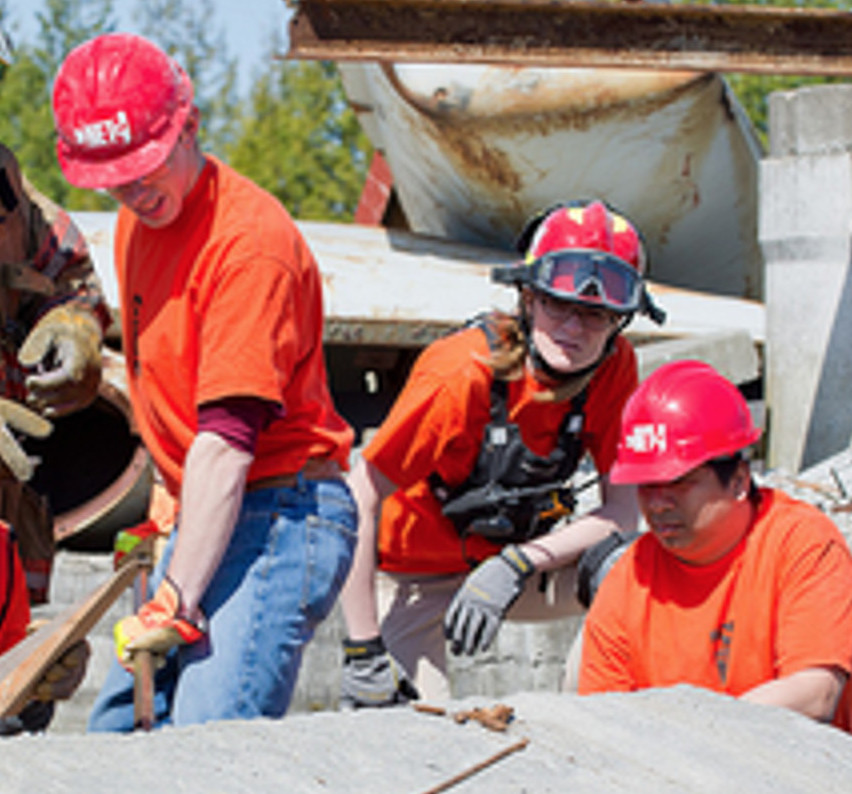
\includegraphics[scale=0.95]{graphics/PortlandNETs2.jpeg}}} % Image background; * means only on this page
\vspace*{6cm}     %from the top of page
\centering{
\normalfont\fontsize{35}{35}\sffamily\selectfont
\textbf{ Retaining Volunteers: \\
Creative Options from the Literature}\\  % Book title
\vspace*{7cm}    % between title and client/author lines
{\LARGE Produced for: \\
Portland Bureau of Emergency Management\\
\vspace*{1cm}   % between client and author
Produced by: \\
Bruce D. Marron \\}  % Author name
} 
\endgroup

%----------------------------------------------------------------------------------------
%	COPYRIGHT PAGE
%----------------------------------------------------------------------------------------

\newpage
~\vfill
\thispagestyle{empty}

\noindent Cover image, \copyright\ Portland NET, 2017\\ % Copyright notice

\noindent Chapter image, \copyright\ Los Angeles County Community Disaster Resilience, 2017\\ % Copyright notice

%\noindent \textsc{Projet Janvier-Mars 2015, Université de Bourgogne}\\

%\noindent Ce projet a été encadré par Hervé CARDOT.\\ % License information

\noindent \textit{Published 10 November 2017} % Printing/edition date

%----------------------------------------------------------------------------------------
%	TABLE OF CONTENTS
%----------------------------------------------------------------------------------------

\chapterimage{graphics/LAResilience.jpeg} % heading image

\pagestyle{empty} % No headers

\renewcommand\contentsname{Table of Contents}
\renewcommand{\bibname}{Bibliography}
\tableofcontents% Print the table of contents itself

%\cleardoublepage % Forces the first chapter to start on an odd page so it's on the right

\pagestyle{fancy} % Print headers again

%%%%%%%%%%%%%%%%%%%%%%%%%%%%%%%%%%%%%%%
%	CHAPTER 1
\chapterimage{graphics/LAResilience.jpeg} % Chapter heading image
\chapter{A Brief Historical Perspective}
%%%%%%%%%%%%%%%%%%%%%%%%%%%%%%%%%%%%%%%%%

\section{Introduction}\index{Introduction}
\vspace{1em}




\vspace{2em}

\section{Portland NET Comes Alive}\index{Portland NET}
\vspace{1em}

  \vspace{1em}


 \vspace{1em}
 




%%%%%%%%%%%%%%%%%%%%%%%%%%%%%%%%%%%%%%%%%%%%%%%
\chapterimage{graphics/LAResilience.jpeg} % Chapter heading image
\chapter{A Brief Look at the Literature}
%%%%%%%%%%%%%%%%%%%%%%%%%%%%%%%%%%%%%%%%%%%%%%%

\section{Literature Highlights}
\vspace{1em}

\autocite{shields_young_2009}\\
Volunteer retention rates are also influenced by several factors perceived by the individual. Specifically, volunteers express high levels of connectedness (feeling part of a group to which one feels they share goals, values, respect, and trust), uniqueness (feeling that one has a unique combination of talents and personality to contribute to the organization), and power (feeling that one can make a difference)\\

young adults have been identified as an under-represented
age group in volunteering . The image of
volunteering may need to be altered to reflect positive and relevant images
to accommodate the needs of young adults. A large proportion of young
people perceive volunteering as not being socially or personally attractive
. Many young adults perceive volunteering as
being boring and involving older people who will not appreciate their skills.
Perceptions such as this need to be overcome as young people represent an
attractive source of volunteers for nonprofit organizations and, thus, are an
important focus for nonprofits’ recruitment efforts . Recognition should be given to the fact that the three most
common barriers to volunteering are lack of time, lack of interest, and ill
health . Young adults would be
particularly venerable to the first two barriers, thus representing a special
recruiting challenge. \\

Decisive research on why people volunteer discovered that
volunteers were motivated by both altruistic and egoistic motives. A widely quoted attempt to categorize volunteering
motivation resulted in six motives for volunteering. Two of the six motives
were related to career and personal enhancement, two were personal development (protective and understanding), 
and two dealt with relationships with others (social and values)\\

Volunteer retention rates
are also influenced by several factors perceived by the individual.
Specifically, volunteers express high levels of connectedness (feeling part
of a group to which one feels they share goals, values, respect, and trust),
uniqueness (feeling that one has a unique combination of talents and
personality to contribute to the organization), and power (feeling that one
can make a difference)\\

Peterson (2004) found that younger volunteers were motivated by
financial and career success and older volunteers were motivated by social
responsibilities and a greater . This study found age to
be the best criteria for selection of recruitment strategies. Australian
researchers, however, concluded that motivations for volunteering did not
differ by age, and that generic promotional and recruitment messages
would be equally effective for all age groups of volunteers\\

Callow (2004) recognized the advantages of
identifying different promotional appeals for targeting the retiree volunteer
segment. Instead of highlighting the similarities within the retiree segment,
Callow advocated future fragmenting the cluster into subgroups.\\

It has already been noted that individuals are often motivated to
volunteer because of egoistic reasons. Young adults are more likely to
volunteer to benefit their own self-interests and concern for their own
personal advancement\\

What promotional appeals for volunteering experiences will subgroups
of young adults find desirable? What are the most appropriate targeting
appeals for this segment? Do the motivations of young adult volunteers differ
from retiree volunteers significantly enough to warrant separate appeals?
How likely and when are young adults to volunteer? Can young adults with
particular desirable traits be recruited with the generic appeals?\\

An eight-item scale by Raskin and
Terry (1988) was used to measure the degree to which one views oneself as
a leader and desires to have influence over others\\

were more likely to volunteer out of egoism (less altruistic)
self-interest, a measure of concern for personal advancement included was
one of four components of vanity. Achievement concern was measured by
Netemeyer, Burton and Lichtenstein’s (1995) five-item scale. This variable
was included to capture a sense of personal enhancement and achievement.\\

Deeming positive attitudes towards working in a team and cooperative
behavior toward others as desirable traits for volunteers, Oliver and
Anderson’s (1994) five-item acceptance (teamwork/cooperation) scale was
included in the study.\\

Three components of mentoring, ability, and willingness (rapport
ability, support willingness, and relational willingness) were considered
admirable traits for potential volunteers and were measured by Pullins et al.’s
(1996) 15-item scale.\\

The promotional appeals that Callow identified for targeting potential retiree
volunteers proved to be effective for segmenting the young adult market, as
well. The four different appeals, based on high and low humanitarian and
social motivations, proved to be attractive to the students in the study\\

By appealing to and targeting subgroups with different motivations
individually, the maximum marketing efficiency can be reached within the
overall segment. Recruitment communications by nonprofit organizations
directed to young adults should highlight and emphasize the following types
of themes and positioning strategies, for instance:
When you volunteer at XYZ nonprofit organization...
...you will actively participate in important activities that make a
difference.
...you will have the opportunity to better yourself personally and
professionally.
...you will make a difference in the lives of others.
...you will make connections with others.\\

The volunteer market, in general, and regardless of life-stage, appears
to be motivated by a combination of humanitarianism and social factors.
Thus appeals to the young adult segment should emphasize these distinct
themes in a format that addresses the specific interests of the cohort groups
such as self-advancement and personal development, since efforts should be
made to accommodate the preferences and imperatives of young people to
be most effective\\

Given that almost a third
of the segment indicated that they are very likely to volunteer in the future, a
carefully executed marketing strategy can be instrumental in attracting and
recruiting the energetic and talented young adult segment who currently
believe they will volunteer in the future. With targeted appeals, the
opportunity to increase volunteerism and capture the energies of the young
adult volunteer segment exists.\\

Considering that professionally employed, college-educated individuals tend
to volunteer in higher numbers than other segments (Wymer, 2003), the fact
that the majority of the respondents had volunteered during their college
experience and felt the need to list volunteering on their resume is not
surprising. Motivation for volunteering is often employment-related.\\

It
would seem young adults can best be recruited by nonprofit organizations if
initial approaches are made, and relationships developed, while the segment
is still in college. The identified humanitarianism/social motivations appear
to apply to multiple life-stages. These appeals combined with the motivation
to start, and establish, a career should prove effective for recruitment efforts.

\vspace{2em}

\section{Literature Summary}
\vspace{1em}


%%%%%%%%%%%%%%%%%%%%%%%%%%%%%%%%%%%%%%%%%%%%%%%%%
\chapterimage{graphics/LAResilience.jpeg} % Chapter heading image
\chapter{A Brief Look at Notable Programs}
%%%%%%%%%%%%%%%%%%%%%%%%%%%%%%%%%%%%%%%%%%%%%%%%%%%%

\section{Program Highlights}
\vspace{1em}




\vspace{2em}

\section{Summary}
\vspace{1em}




\vspace{1em}

%%%%%%%%%%%%%%%%%%%%%%%%%%%%%%%%%%%%%%%%%%%%%%%%%
\chapterimage{graphics/LAResilience.jpeg} % Chapter heading image
\chapter{Creative Options}
%%%%%%%%%%%%%%%%%%%%%%%%%%%%%%%%%%%%%%%%%%%%%%%%%%%%

\section{A Brief List of Creative Options}



\section{Final Recommendations}

% ----------------------------------------------------------------------------------------
% 	BIBLIOGRAPHY
% ----------------------------------------------------------------------------------------
          

\printbibliography



\end{document}
